\section{Potential and Field}

Maxwell Equations

\begin{eqnarray}
\begin{aligned}
    \nabla \cdot \textbf{E}{}&=\frac{\rho}{\epsilon_0}\\
    \nabla \cdot \textbf{B} &= 0\\
    \nabla \times \textbf{E} &= -\frac{\partial \textbf{B}}{\partial t}\\
     \nabla \times \textbf{B} &= \mu_0\textbf{J}+\mu_0\epsilon_0 \frac{\partial \textbf{E}}{\partial t}\\
\end{aligned}
     \label{eq:Maxwell}
\end{eqnarray}

Using vector potential to present magnetic field with Lorentz gauge
\begin{eqnarray}
     \textbf{B}= \nabla \times \textbf{A}\\
     \textbf{E}=-\nabla \phi -\frac{\partial \textbf{A}}{\partial t}\\
     \nabla \cdot \textbf{A}+ \frac{1}{c^2}\frac{\partial \phi}{\partial t}=0
\end{eqnarray}

\section{Ohm's Law}

Ohm's Law

\begin{equation}
    \textbf{E}+\frac{1}{c}\textbf{V}\times \textbf{B}= \frac{1}{\sigma}\textbf{J}
\end{equation}

Since $\left(\frac{1}{c}\textbf{V}\times \textbf{B}
\right)_{||}< O^2$, then 

\begin{equation}
    E_{||} = \frac{1}{\sigma_{||}}J_{||} + O^2
\end{equation}

\section{Doppler shift}

\begin{equation}
f=\left(\frac{c \pm v_{\mathrm{r}}}{c \pm v_{\mathrm{s}}}\right) f_{0}
\end{equation}

For $v_r \ll c$ 

\section{Pressure tensor}
In section 3.2.5 of Principle of plasma physics by Krall \cite{Principle}.
\begin{equation}
    P_\alpha(\textbf{x},t)=\bar{n}_\alpha m_\alpha\int (\textbf{v}-\textbf{V}_\alpha)(v-\textbf{V}_\alpha)f_\alpha(\textbf{x},\textbf{v},t)d\textbf{v}
\end{equation}


\section{Magnetic pressure}

Magnetic pressure can be expressed as $P_{B}=\frac{B^{2}}{8 \pi}$


\section{Ballooning transformation}

Since the poloridal and toroidal angel $\theta \in (-\infty, \infty)$, for convenience. we define a function

\begin{equation}
z(\theta)=\sum_{l=-\infty}^{\infty} \bar{z}(\theta+2 \pi l)
\end{equation}

So all the function on the same location with but different winding times added together. 

\section{$(\phi,\zeta ,\chi)$}

$\phi$ is the radius-like coordinate, same $\phi$ means same magnetic surface. $\zeta$ is toroidal angle-like coordinate, $\chi$ is poloidal angle-like coordinate. \cite{Ballooning_transformation}

\section{MHD approximation}



\section{Gyro-average\label{sec:gyro}}

\subsection{Overview}
A great resource for gyro-average is the early paper of GENE\cite{merz} "Integrals for the field equations"

\begin{equation}
A(\vec{X}+\vec{r})=\sum_{k_{x}, k_{y}} A\left(k_{x}, k_{y}\right) e^{i \vec{k}_{\perp} \cdot(\vec{X}+\vec{r})}
\end{equation}
\begin{equation}
\begin{aligned}
    A(\textbf{x})
    {}&\longrightarrow< A(\textbf{X})>=A\left(k_{x}, k_{y}\right)J_0(k_\perp \rho_s)\\
    &\longrightarrow< A(\textbf{x})>=A\left(k_{x}, k_{y}\right)J_0^2(k_\perp \rho_s)\\
    &\longrightarrow A(\textbf{k})=A(\textbf{x})J_0(k_\perp \rho_s)
    \end{aligned}
\end{equation}


\subsection{Derivation}

For helix motion, we have

\begin{eqnarray}
    \Vec{x}= \rho_s cos(\omega t)\hat{x}+\rho_s sin(\omega t)\hat{y}+ x_{c} \hat{z}\\
    \omega =\frac{qB}{m}\\
    \rho_s=\frac{mv}{q_sB}
\end{eqnarray}

Where $x_{c}$ is the guiding center of the particle.

For any quantities that depends on the trajectory of charged particles will be taken average over gyro-radius. The following average method only works for $\frac{\omega}{\omega_g}\ll 1$ frequency of the of mode less than the gyro-frequency. The mode frequency is so slow that for a period of gyro-motion, the quantity of interest will stay constant.

The gyro-average of a scalar field can be written as

\begin{equation}
\begin{aligned}\langle A(X)\rangle &=\frac{1}{2 \pi} \int_{0}^{2 \pi} A(\vec{X}+\vec{r}) d \theta=\frac{1}{2 \pi} \int_{0}^{2 \pi} \sum_{k_{x}, k_{y}} A\left(k_{x}, k_{y}\right) e^{i \vec{k}_{\perp} \cdot(\vec{X}+\vec{r})} d \theta \\ 
&=\sum_{k_{x}, k_{y}} A\left(k_{x}, k_{y}\right) e^{i \vec{k}_{\perp} \cdot \vec{X}} \frac{1}{2 \pi} \int_{0}^{2 \pi} e^{i \vec{k}_{\perp} \cdot \vec{r}} d \theta \\
&=\sum_{k_{x}, k_{y}} A\left(k_{x}, k_{y}\right) e^{i \vec{k}_{\perp} \cdot \vec{X}} \frac{1}{2 \pi} \int_{0}^{2 \pi} e^{ik_{\perp} r cos\theta} d \theta \\
&=\sum_{k_{x}, k_{y}} A\left(k_{x}, k_{y}\right) e^{i \vec{k}_{\perp} \cdot \vec{X}} J_{0,s}(k_{\perp}\rho )\\
\end{aligned}
\label{eq:gyro_avg}
\end{equation}

Where $J_{0,s}(k_{\perp}\rho )=\frac{1}{2\pi} \int d \theta e^{ik_{\perp}\rho_s cos \theta}$. Therefore gyro-average introduces a $J_{0,s}(k_{\perp}\rho )$. Here is a plot of $J_0$ shown on Figure \ref{fig:J0}

\begin{figure}[h] \centering
        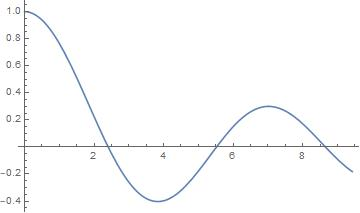
\includegraphics[width=0.5\textwidth]{Image/J0.jpg}
        \caption{Plot of Bessel function of first kind $J_0(x)$}
        \label{fig:J0}
    \end{figure}

From the guiding center to the real space is \cite{merz}

\begin{equation}
\begin{aligned}\langle\overline{A}(\vec{x}-\vec{r})\rangle &=\frac{1}{2 \pi} \int_{0}^{2 \pi} \frac{1}{2 \pi} \int_{0}^{2 \pi} A\left(\vec{x}-\vec{r}+\vec{r}^{\prime}\right) d \theta d \theta^{\prime} \\ &=\frac{1}{4 \pi^{2}} \int_{0}^{2 \pi} \int_{0}^{2 \pi} \sum_{k_{x}, k_{y}} A\left(k_{x}, k_{y}\right) e^{i \vec{k}_{\perp} \cdot\left(\vec{X}-\vec{r}+\vec{r}^{\prime}\right)} d \theta d \theta^{\prime} \\ &=\sum_{k_{x}, k_{y}} A\left(k_{x}, k_{y}\right) e^{i \vec{k}_{\perp} \cdot \vec{X}} J_{0}^{2}\left(\rho k_{\perp}\right) \end{aligned}
\end{equation}

For a velocity that is changing with frequency of gyro frequency, curvature drift velocity for instance, \cite{Vd} \cite{iter_scale}

\begin{equation}
    \begin{aligned}
        <\Tilde{v}^2_{\perp}>{}&=<v^2_{\perp}cos^2(\omega t)>\\
        &=\frac{\omega}{2\pi}\int^{\frac{2\pi}{\omega} }_{0}v^2_{\perp}cos^2(\omega t) dt\\
        &=\frac{1}{2} v^2_{\perp}
    \end{aligned}
\end{equation}

    
\section{Quasi-neutrality}

The assumption of quasi-neutrality is based on low oscillation frequency of the mode of interest compared with plasma frequency. 

\begin{equation}
    \frac{\omega}{\omega_p} \ll 1
\end{equation}

\section{Curl}
    For the Vector in the form of $\widetilde{\textbf{A}}=\textbf{A} e^{i\textbf{kx}-i\omega t}$. We can calcuate the curl as shown below. Where $A$ is a constant in terms of time and position. 
    \begin{eqnarray}
        \nabla \times (f\textbf{A}) = f \nabla \times \textbf{A} +(\nabla f)\times \textbf{A}\\
        \nabla \times (e^{i\textbf{kx}-i\omega t}\textbf{A}) = e^{i\textbf{kx}-i\omega t} \nabla \times \textbf{A} +(\nabla e^{i\textbf{kx}-i\omega t})\times \textbf{A}\\
        \nabla \times \widetilde{\textbf{A}}=  i\textbf{k} \times \widetilde{\textbf{A}}
    \end{eqnarray}
    Assuming $\textbf{A}=A\hat{z}, \textbf{k}=k\hat{y}$
    \begin{eqnarray}
    \begin{aligned}
        \textbf{B}e^{i\textbf{kx}-i\omega t}{}&= i\textbf{k}\times \widetilde{\textbf{A}}\\
        &=ik A e^{i\textbf{kx}-i\omega t}\hat{x}
        \label{eq:curl}
    \end{aligned}
    \end{eqnarray}
    
Based on Maxwell's equations:

\begin{eqnarray}
\begin{aligned}
    \nabla \textbf{E}{}&=\frac{\rho}{\epsilon_0}\\
    \nabla \textbf{B} &= 0\\
    \nabla \times \textbf{E} &= -\frac{\partial \textbf{B}}{\partial t}\\
     \nabla \times \textbf{B} &= \mu_0\textbf{J}+\mu_0\epsilon_0 \frac{\partial \textbf{E}}{\partial t}\\
\end{aligned}
     \label{eq:Maxwell}
\end{eqnarray}
Using vector potential to present magnetic field with Lorentz gauge
\begin{eqnarray}
     \textbf{B}= \nabla \times \textbf{A}\\
     \textbf{E}=-\nabla \phi -\frac{\partial \textbf{A}}{\partial t}\\
     \nabla \textbf{A}+ \frac{1}{c^2}\frac{\partial \phi}{\partial t}=0
\end{eqnarray}

Therefore we can express magnetic field and electric field as following way:
\begin{eqnarray}
     \textbf{B}= i\textbf{k}\times \textbf{A}\\
     \textbf{E} = -i\textbf{k} \phi +i\omega \textbf{A}
     \label{eq:E-A}
\end{eqnarray}

\begin{eqnarray}
     \nabla \times (\nabla \times \textbf{A})=\nabla (\nabla \textbf{A}) -\nabla^2 \textbf{A}\\
     \nabla^2 \textbf{A}=\frac{\omega^2}{c^2} \textbf{A}-\frac{4\pi}{c} \textbf{J}\\
     (k^2-\frac{\omega^2}{c^2})A_{||}=-\frac{4\pi}{c}J_{||}\\
    \nabla \times (\nabla \times \textbf{A})=\frac{4\pi}{c} \textbf{J}
\end{eqnarray}

\section{Common Quantities}

\subsection{Toroidal coordinates}
For the simplicity, plasma physicists use toroidal coordinates. We define the following quantities.

Here is the coordinate $(r, \phi, \theta)$. 

\begin{eqnarray}
\begin{aligned}
    R=major\ radius\\
    r= minor\ radius\\
    \zeta=\phi= toroidal\ angle\\
    \theta = poroidal\ angle
\end{aligned}
\end{eqnarray}

\subsection{Shafranov shift}

\begin{eqnarray}
     \begin{aligned}
      r’{}&=R_0+\Delta(r)-r cos\alpha\\
      \theta’&=\zeta\\
      z’&=r sin\alpha=r sin(\theta+\delta)
     \end{aligned}
\end{eqnarray}

\subsection{Flux coordinates}

Flux coordinates can be express in the following fashion: $(\psi, \chi, \zeta)$

Where $\psi$ is magentic flux, which is defined as 

\begin{eqnarray}
\begin{aligned}
   \phi_p{}&=\int \textbf{B}_Td\textbf{s}\\
   \phi_T&=\int \textbf{B}_Pd\textbf{s}\\
\end{aligned}
\end{eqnarray}

Since magnetic field is pointing at the same direction with varying radius, The magnitude of magnetic flux is monotonically increasing, that means one can map the magnetic flux to radius is a one-to-one manner. 

\subsection{Wave number}
The wave number in GENE refers to the magnetic field, which can be considered as operator 

\begin{eqnarray}
\begin{aligned}
    k_{||}{}&=-i\nabla_{||}\\
    &=-i\textbf{b}\cdot \nabla \\
    &=-i\frac{B_z}{B_0}(\hat{e}_{\zeta}+\frac{r}{qR}\hat{e}_{\theta})\cdot(\hat{e}_{r}\frac{\partial}{\partial r}+\hat{e}_{\theta}\frac{1}{r}\frac{\partial}{\partial \theta}+\frac{1}{R}\hat{e}_{\zeta}\frac{\partial}{\partial \zeta})\\
    &=-i\frac{B_z}{B_0}(\frac{1}{qR}\frac{\partial}{\partial \theta }+\frac{1}{R}\frac{\partial}{\partial \zeta})\\
    &= -i \frac{B_z}{B_0}\frac{1}{qR}(\frac{\partial}{\partial \theta }+q\frac{\partial}{\partial \zeta})
\end{aligned}
\end{eqnarray}

If we apply this operator to a wave function $\phi=\phi(r)e^{im\theta -in \zeta }\sum_l e^{i l\theta}$
For slab geometry, $l=0$, therefore, we have the following equation,

\begin{eqnarray}
\phi=e^{im\theta -in \zeta }\\
k_{||}\phi = \frac{B_z}{B_0}\frac{1}{qR}(m - qn)\phi
\end{eqnarray}

From $k_{||}$, one can get $k_{\perp}$ 

\begin{eqnarray}
\begin{aligned}
\nabla_{\perp}{}&=\nabla -\nabla_{||}\\
%&=(\hat{b}\nabla)\hat{b}-(\hat{b} \cdot \hat{b})\nabla\\
%&=\hat{b}\times(\hat{b}\times \nabla)\\
&=\hat{e}_{r}\frac{\partial}{\partial r}+\hat{e}_{\theta}\frac{1}{r}\frac{\partial}{\partial \theta}-\frac{1}{qR}\hat{e}_{\zeta}\frac{\partial}{\partial \theta}
\end{aligned}
\end{eqnarray}

Since $\frac{r}{R}\ll 1$, then it is valid to drop the third term. Therefore, we have:

\begin{eqnarray}
\nabla_{\perp}=\hat{e}_{r}\frac{\partial}{\partial r}+\hat{e}_{\theta}\frac{1}{r}\frac{\partial}{\partial \theta}
\end{eqnarray}

Then we have (In GENE coordinates)

\begin{eqnarray}
\begin{aligned}
k_{x}{}&=-i\frac{\partial}{\partial r}\\
k_{y}&=-i\frac{1}{r}\frac{\partial}{\partial \theta}\\
k_z&=k_{||}=-i \frac{1}{qR}(\frac{\partial}{\partial \theta }+q\frac{\partial}{\partial \zeta})
\end{aligned}
\end{eqnarray}

Plug $k_x$ and $k_y$ into $\phi=e^{im\theta -in \zeta }$\\

\begin{eqnarray}
\begin{aligned}
k_{x}\phi{}&=-i\frac{\partial}{\partial r}\phi\\
k_{y}\phi&=\frac{m}{r}\phi\\
k_{z}\phi&=k_{||}\phi= \frac{m-nq}{qR}\phi
\label{eq:k_slab}
\end{aligned}
\end{eqnarray}

For the most cases, $\frac{r}{\rho_s}=500$. Where $\rho_s$ is the gyro-radii. So if $k_y\rho_s$ is smaller than 0.02, then we are in region that m is in the order of 10. then $k_y\rho_s$ is will be less continuous since m has to be a integer. 

\subsection{Bootstrap current}

The Bootstrap current is induced by $\frac{\nabla p \times B_p}{B}$ where $B_p$ is the poloridal magnetic field. From the Wesson's book Tokamaks \cite{Tokamaks}


\begin{equation}
j_{\mathrm{b}}=-\frac{\varepsilon^{1 / 2} n}{B_{\theta}}\left[2.44\left(T_{\mathrm{e}}+T_{\mathrm{i}}\right) \frac{1}{n} \frac{\mathrm{d} n}{\mathrm{d} r}+0.69 \frac{\mathrm{d} T_{\mathrm{e}}}{\mathrm{d} r}-0.42 \frac{\mathrm{d} T_{\mathrm{i}}}{\mathrm{d} r}\right]
\end{equation}

The bootstrap current will induce magnetic field that is opposite the $B_p$. That is the the reason why the pedestal region where the pressure gradient is high. The magnetic shear is small. As the the Figure\ref{fig:j_bs} shows. 

\begin{figure}[h] \centering
        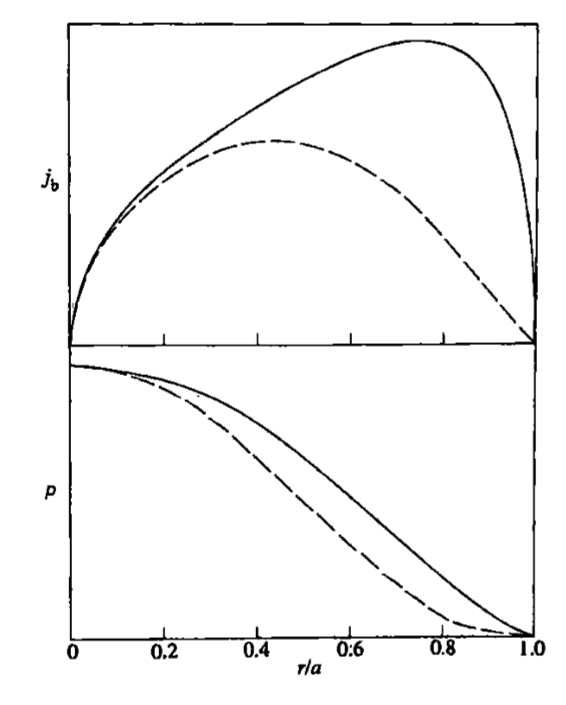
\includegraphics[width=1\textwidth]{Image/BS_current.png}
        \caption{Bootstrap current distribution in radius}
        \label{fig:j_bs}
\end{figure}


The origin of the bootstrap current comes from the the idea that bootstrap current will be one of the component that will make the fusion devices self-sustainable. 


\subsection{safety factor and rational surface}

\subsubsection{Safety factor}

Safety factor can be understood as "twistiness of the magnetic field", which can be expressed as 

\begin{eqnarray}
q=\frac{B_{tor}}{2\pi R} (\frac{B_{por}}{2\pi r})^{-1}
\end{eqnarray}

One can also think that $\frac{2\pi}{q}$ is how much the magnetic field have turned after a turn toroidally or $q=\frac{d \phi}{d \theta}$

\subsubsection{Rational surface}

Rational surface is the surface when q is rational e.g. q can be expressed as  $q=\frac{m}{n}$.That means it takes n turns toroidally, and m turns poroidally to get back to the original spot.  n is the toroidal mode number, m is the poloidal mode number




\section{Dedye shielding \label{sec:debye}\cite{Chen}}

From 1-D Poisson's Equation:

\begin{eqnarray}
\frac{\partial^2 \phi}{\partial x^2} =-4\pi e(n_i-n_e)
\end{eqnarray}

With the potential of $q\phi$ and the kinetic energy $\frac{1}{2}mv^2$, we have the distribution function as following:

\begin{equation}
f(v)=A \exp \left[-\left(\frac{1}{2} m v^{2}+q \phi\right) / T_{e}\right]
\end{equation}

The distance of a ion to a ion is much further than electron, i.e. $r_i\gg r_e$. $f_i \approx A\exp[-\frac{m_iv^2}{2T_e}]$

With the relationship of density and distribution function: 

\begin{eqnarray}
 n_s=\int f(v) dv\\
 n_i=n_0\\
 n_e=n_0 \exp (e\phi/T_e)\\
 \rho_{tot}=-e(n_i-n_e)=en_0[\exp (e\phi/T_e)-1]\label{eq:neutral}
\end{eqnarray}


We can expand the distribution function in terms of $\frac{e\phi}{T_e}$ if $\frac{e\phi}{T_e}\ll 1$

\begin{eqnarray}
 \nabla^2 \phi = -\rho_{tot}\\
 \frac{\partial^2 \phi}{\partial x^2}=4\pi en_0[(e\phi/T_e)+\frac{1}{2}(e\phi/T_e)^2+...]
\end{eqnarray}

Take the first order of the Taylor Expansion, can solve this differential equation with ease,

\begin{equation}
    \phi=\phi_0e^{\pm x\sqrt{\frac{4\pi n_0e^2}{T_e}}}
\end{equation}

For the sake of convergence, we left with only one solution, 

\begin{equation}
    \phi=\phi_0e^{- x\sqrt{\frac{4\pi n_0e^2}{T_e}}}
\end{equation}

Define Debye length $\lambda_D=\sqrt{\frac{T_e}{4\pi n_0e^2}}$, then we have

\begin{equation}
     \phi=\phi_0e^{-x/\lambda_D}
\end{equation}

The physical understanding of Debye length is that beyond which length, charged particle will not experience the significant amount of electric field. 

Quasi neutrality can be implied from the derivation above, From Equation \ref{eq:neutral}, we can see that $\rho_{tot} \approx 0$ which is quasi neutral. Therefore we can will have the following conclusion 

\begin{eqnarray}
 \frac{e\phi}{T_e}\ll 1 \Longrightarrow \rho_{tot} \approx 0
\end{eqnarray}

$1_{st}$ order adiabatic perturbation can be implied from it as well, the distribution function can be expanded

\begin{equation}
    f_e=Ae^{-\frac{mv^2}{2T}}[1+(\frac{q\phi}{T_e})+\frac{1}{2}(\frac{q\phi}{T_e})^2+...]
\end{equation}

The first term is $0_{th}$ order - Maxwellian distribution, second term is the $1_{st}$ order adiabatic perturbed term.

\subsection{Adiabatic perturbed term}

Let's assume we have the magnetic term in the adiabatic perturbed term.Similar to the Debye shielding, we can use the Hamiltonian to derive the adiabatic perturbed term. 

\begin{equation}
\begin{aligned}
    f{}&=F_0\left(1+\frac{q_s\textbf{v}\cdot \textbf{A}}{cT_s}-\frac{q_s\phi}{T_s} \right)+h_s\\
    &=F_0+\delta f
\end{aligned}
\end{equation}

Where $F_0$ is the Maxwellian distribution, $F_0\left(\frac{q_s\textbf{v}\cdot \textbf{A}}{cT_s}-\frac{q_s\phi}{T_s} \right)$ is adiabatic perturbed term, $h_s$ is the non-adiabatic perturbed term

Plug into Equation\ref{eq:temp23}, 

\begin{equation}
\begin{aligned}
    (\omega -\omega_D 
    - k_{||}v_{||})\left[F_0\left(\frac{q_sA_{||}v_{||}}{cT_s}-\frac{q_s\phi}{T_s} \right)+h_s\right]
    +\\
    \left[\omega_{*}^{tot}\frac{q_s\phi}{T_s}+
    (\omega-\omega^{tot}_*) \frac{q_s A_{||}v_{||}}{cT_s}-(k_{||}v_{||}+\omega_D)\frac{q_s\phi}{T_s}\right]F_0
    =i\left(\frac{\partial f}{\partial t}\right)_{\mathrm{coll}}
\end{aligned}
\end{equation}

After some algebra, we are left with

\begin{equation}
     (\omega -\omega_D 
    - k_{||}v_{||})h_s 
    -(\omega -\omega_*^{tot})\frac{q_s\phi}{T_s}F_0+(2\omega -\omega^{tot}-\omega_D-k_{||}v_{||})\frac{q_sA_{||}v_{||}}{cT_s}F_0
    =i\left(\frac{\partial f}{\partial t}\right)_{\mathrm{coll}}
\end{equation}

If we assume $i\left(\frac{\partial f}{\partial t}\right)_{\mathrm{coll}} = -i\nu(h_s) h_s$, then we can obtain the following expression

\begin{equation}
    h_s 
    =\frac{\omega -\omega_*^{tot} 
    }{\omega -\omega_D 
    - k_{||}v_{||}+i\nu(h_s)}\left(\frac{q_s\phi}{T_s}-\frac{q_sA_{||}v_{||}}{cT_s}\right)F_0 - \frac{q_sA_{||}v_{||}}{cT_s}F_0
    \label{eq:linear2}
\end{equation}

When it is effectively 

\begin{equation}
    \delta f =-\frac{q_s\phi}{T_s}F_0+h_s
    \label{eq:adiabatic}
\end{equation}

Where $
    h_s 
    =\frac{\omega -\omega_*^{tot} 
    }{\omega -\omega_D 
    - k_{||}v_{||}+i\nu(h_s)}\left(\frac{q_s\phi}{T_s}-\frac{q_sA_{||}v_{||}}{cT_s}\right)F_0
$

\subsection{$Delta$(Delta)}

From \cite{tearing_parity} Appendix, the explanation was given for $Delta$. 



\section{Maxwellian distribution}

The origin of Maxwellian distribution ($\sqrt{\frac{m}{2\pi  T}}e^{-\frac{mv^2}{2T}}$)can be traced back to the Boltzmann distribution ($p\propto e^{-\frac{\epsilon}{T}}$) microscopic statistical mechanics. However, one can derive Maxwellian distribution from Boltzmann Equation with no force. 

From collisional plasma physics point of view, the\textbf{ H theorem} will be the answer to the equilibrium distribution being Maxwellian. 

\begin{equation}
    \frac{\partial f}{\partial t} +\Vec{v} \nabla f +\Vec{F}\frac{\partial f}{\partial \epsilon}=(\frac{\partial f}{\partial t})_{coll}
\end{equation}

For the future reference, we can examine it by plugging in the Maxwellian equation$F_0=\sqrt{\frac{m}{2\pi T}}e^{-\frac{mv^2}{2T}}$

\begin{eqnarray}
 \frac{\partial F_0}{\partial t}=0\\
 \frac{\partial F_0}{\partial \epsilon}=\frac{1}{T}F_0\\
 \nabla F_0 = \left[\frac{\nabla n_0}{n_0}+(\frac{3}{2}-\frac{mv^2}{2T})\frac{\nabla T_0}{T_0}\right]F_0\\
 \vec{F}=q(\vec{E}+\vec{v}\times \vec{B})\\
 \vec{v}_{||}\nabla F_0=0
\end{eqnarray}

Where force is negligible. The density and temperature change along the field line is small. 

\section{Gaussian Unit \label{sec:gauss}}

Maxwell's Equations

\begin{equation}
\begin{array}{l}
{\nabla \cdot \mathbf{E}=4 \pi \rho} \\ 
{\nabla \cdot \mathbf{B}=0} \\ 
{\nabla \times \textbf{E} = -\frac{1}{c}\frac{\partial \textbf{B}}{\partial t}}\\
{\nabla \times \mathbf{B}=\frac{4 \pi}{c} \mathbf{J}+\frac{1}{c} \frac{\partial \mathbf{E}}{\partial t}}
\end{array}
\end{equation}

And $k_B=1$

Here are some good quantities

\begin{eqnarray}
 v_E=\frac{E_{SI}}{B_{SI}}=\frac{1}{c}\frac{E_G}{B_G}
\end{eqnarray}

Here is the conversion from SI unit to Gauss Unit\cite{Handbook}

\begin{equation}
\begin{array}{lll}{\epsilon_{0} \mapsto 1 /(4 \pi)} & {\mu_{0} \mapsto 4 \pi / c^{2}} & {B \mapsto B / c} \\ {\chi_{E} \mapsto 4 \pi \chi_{E}} & {\chi_{H} \mapsto 4 \pi \chi_{H}} & {H \mapsto c H /(4 \pi)} \\ {A \mapsto A / c} & {M \mapsto c M} & {D \mapsto D /(4 \pi)}\end{array}
\end{equation}

A good place to check it Wikipedia 

\begin{verbatim}
    https://en.wikipedia.org/wiki/Gaussian_units
\end{verbatim}

\section{Ordering}

$R_c$ is the curvature of the device which is in the order of the major radius of the device. 

$r_g$ is the gyro-radius.Commonly, magnetic field is the order of 5T. 

\begin{equation}
    \begin{aligned}
    R_c ~ 5m
    r_g=\frac{mv_{\perp}}{qB} ~ 1cm
    \end{aligned}
\end{equation}

With ordering law of the 

\begin{equation}
\begin{aligned}
v_D{}&=\left(v_{ \|}^{2}+\frac{1}{2} v_{\perp}^{2}\right) \frac{m}{q} \frac{\mathbf{R}_{c} \times \mathbf{B}}{R_{c}^{2} B^{2}}\\
\frac{v_D}{v_{||}}&\approx \frac{v_{||} m}{R_cB_0q}\\
\frac{v_D}{v_{||}}&\approx \frac{v_{||}}{v_{\perp}}\frac{r_g}{R_c}
\label{eq:vD}
\end{aligned}
\end{equation}

\section{Collision\cite{coll}}\label{sec:coll}

Define $\hat{c}=\frac{\textbf{g}_f-\textbf{g}_i}{|\textbf{g}_f-\textbf{g}_i|}$, where $\textbf{g}=\textbf{v}_1-\textbf{v}_2$. f stand for final, i stands for initial. 

\begin{equation}
    \hat{c}=cos\left(\frac{\chi}{2}\right)(cos\phi \hat{x}_i+sin\phi \hat{y}_i)-sin\left(\frac{\chi}{2}\right)\frac{\textbf{g}_i}{g_i}
\end{equation}

As figure \ref{fig:coll1} shown, $\chi$ is the angle between $\textbf{g}_i$ and $\textbf{g}_f$

\begin{figure}[h] \centering
        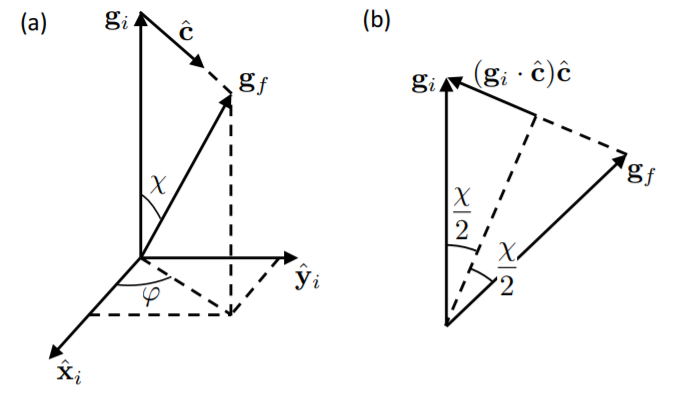
\includegraphics[width=1\textwidth]{Image/coll1.PNG}
        \caption{Diagram of the setup of binary collision}
        \label{fig:coll1}
\end{figure}

We define the following relation

\begin{equation}
\mathbf{g}_{f}=\underline{\mathbf{g}}_{i} \equiv(\mathbf{I}-2 \hat{\mathbf{c}} \hat{\mathbf{c}}) \cdot \mathbf{g}_{i}
\end{equation}

Then we have

\begin{equation}
\mathbf{g}_{i}=\mathbf{g}_{f} \equiv(\mathbf{I}-2 \hat{\mathbf{c}} \hat{\mathbf{c}}) \cdot \mathbf{g}_{f}
\end{equation}

\begin{equation}
\underline{\underline{g}_{i}}=(\mathbf{I}-2 \hat{\mathbf{c}} \hat{\mathbf{c}}) \cdot(\mathbf{I}-2 \hat{\mathbf{c}} \hat{\mathbf{c}}) \cdot \mathbf{g}_{i}=[\mathbf{I}-4 \hat{\mathbf{c}} \hat{\mathbf{c}}+4(\hat{\mathbf{c}} \cdot \hat{\mathbf{c}}) \hat{\mathbf{c}} \hat{\mathbf{c}}] \cdot \mathbf{g}_{i}=\mathbf{g}_{i}
\end{equation}

Define $Q=\mathbf{I}-2 \hat{\mathbf{c}} \hat{\mathbf{c}}$

Here is heuristic derivation from BBGKY approach \cite{coll2}. 

\begin{equation}
\begin{array}{l}{\int X(\mathbf{r}, \mathbf{v}, t) C_{s s^{\prime}}\left[f_{s}, f_{s^{\prime}}\right](\mathbf{r}, \mathbf{v}, t) \mathrm{d}^{3} v=} \\ {\int \mathrm{d}^{3} v f_{s}(\mathbf{v}) \int \mathrm{d}^{3} v^{\prime} f_{s^{\prime}}\left(\mathbf{v}^{\prime}\right) \int_{0}^{2 \pi} \mathrm{d} \varphi \int_{0}^{\pi} \mathrm{d} \chi g \sigma_{s s^{\prime}}(g, \chi) \sin \chi[X(\underline{\mathbf{v}})-X(\mathbf{v})]}\end{array}
\end{equation}

Where $X$ is any function, $\sigma$ is cross section $\sigma_{s s^{\prime}}=\frac{\rho}{\sin \chi}\left|\frac{\partial \rho}{\partial \chi}\right|$.

\subsection{Coulomb collisions}

With potential 

\begin{equation}
V(r)=\frac{Z_{s} Z_{s^{\prime}} e^{2}}{4 \pi \epsilon_{0} r}
\end{equation}

Apply conservation of energy and angular momentum

\begin{equation}
\begin{aligned} \frac{\mathrm{d} r}{\mathrm{d} \theta}=\frac{\mathrm{d} r / \mathrm{d} t}{\mathrm{d} \theta / \mathrm{d} t} &=\pm \frac{r^{2}}{\rho} \sqrt{1-\frac{2 b_{s s^{\prime}}}{r}-\frac{\rho^{2}}{r^{2}}}
\end{aligned}
\end{equation}

Where $b_{s s^{\prime}}=\frac{Z_{s} Z_{s}^{\prime} e^{2}}{4 \pi \epsilon_{0} \mu_{s s^{\prime}}^{\prime} g^{2}}$

After integration, we have Rutherford cross section

\begin{equation}
\sigma_{s s^{\prime}}=\frac{b_{s s^{\prime}}^{2}}{4 \sin ^{4}(\chi / 2)}
\end{equation}

\subsection{Fokker-Planck collision operator}

If we assume $\chi \ll 1$ then we have

\begin{equation}
\sigma_{s s^{\prime}} \simeq \frac{4 b_{s s^{\prime}}^{2}}{\chi^{4}}
\end{equation}

We ended up with the Landau form of Fokker-Planck
collision operator

\begin{equation}
C_{s s^{\prime}}\left[f_{s}, f_{s^{\prime}}\right]=\frac{\gamma_{s s^{\prime}}}{m_{s}} \nabla_{v} \cdot\left\{\int \nabla_{g} \nabla_{g} g \cdot\left[\frac{f_{s^{\prime}}\left(\mathbf{v}^{\prime}\right)}{m_{s}} \nabla_{v} f_{s}(\mathbf{v})-\frac{f_{s}(\mathbf{v})}{m_{s^{\prime}}} \nabla_{v^{\prime}} f_{s^{\prime}}\left(\mathbf{v}^{\prime}\right)\right] \mathrm{d}^{3} v^{\prime}\right\}
\end{equation}

With H-theorm

\begin{equation}
\dot{\sigma}_{s s^{\prime}}+\dot{\sigma}_{s^{\prime} s} \geqslant 0
\end{equation}

Where $\dot{\sigma}_{s s^{\prime}}=-\int \ln f_{s}(\mathbf{r}, \mathbf{v}, t) C_{s s^{\prime}}\left[f_{s}, f_{s^{\prime}}\right](\mathbf{r}, \mathbf{v}, t) \mathrm{d}^{3} v$
and $\dot{\sigma}_{s s^{\prime}}+\dot{\sigma}_{s^{\prime} s}$ is equal to zero only when both $f_{s}$ and $f_{s^{\prime}}$ are Maxwellians with the same
average velocity $\mathbf{u}$ and temperature $T$.

The H-theorem of the Fokker-Planck collision operator implies that the only solutions
to the system of equations 

\begin{equation}
\begin{array}{l}{C_{s s^{\prime}}\left[f_{s}, f_{s^{\prime}}\right]=0} \\ {C_{s^{\prime} s}\left[f_{s^{\prime}}, f_{s}\right]=0}\end{array}
\end{equation}

are the Maxwellian

\subsection{Krook Collation Operator}

Let's start from lineariezed Fokker Plank collision operator between electron and ion: Equation 24 in \cite{MTM_RH}, 

\begin{equation}
C_{e i}^{l}=\frac{3 \sqrt{\pi}}{4 \tau} v_{t_{e}}^{3}\left(\frac{1}{2 v^{3}} \frac{\partial}{\partial \zeta}\left(1-\zeta^{2}\right) \frac{\partial f_{1 e}}{\partial \zeta}+\frac{2 V_{|| i} \zeta}{v_{t_{e}}^{2} v^{2}} f_{M_{e}}\right)
\label{eq:linear_coll}
\end{equation}

Where $\zeta \equiv v_{n} / v$ is the cosine of the pitch angle. 

Recall Legendre differential equation

\begin{equation}
\frac{d}{d x}\left[\left(1-x^{2}\right) \frac{d y}{d x}\right]+l(l+1) y=0
\label{eq:legendre_diff}
\end{equation}

whose solutions are Legendre polynomials

\begin{equation}
\begin{array}{l}{P_{0}(x)=1} \\ {P_{1}(x)=x} \\ {P_{2}(x)=\frac{1}{2}\left(3 x^{2}-1\right)} \\ {P_{3}(x)=\frac{1}{2}\left(5 x^{3}-3 x\right)} \\ {P_{4}(x)=\frac{1}{8}\left(35 x^{4}-30 x^{2}+3\right)} \\ {P_{5}(x)=\frac{1}{8}\left(63 x^{5}-70 x^{3}+15 x\right)} \\ {P_{6}(x)=\frac{1}{16}\left(231 x^{6}-315 x^{4}+105 x^{2}-5\right)}\end{array}
\label{eq:legendre_poly}
\end{equation}

If the perturbed term can be expressed in terms of the eigenfunctions of Legendre differential equation, such that $f_{1e}=\sum a_ly_l(\zeta)$, then the first term of Equation\ref{eq:linear_coll} can be simplified

\begin{equation}
C_{e i}^{l}=\frac{3 \sqrt{\pi}}{4 \tau} v_{t_{e}}^{3}\left(-\frac{1}{2 v^{3}} 
\sum l(l+1)a_ly_l(\zeta)
+\frac{2 V_{|| i} \zeta}{v_{t_{e}}^{2} v^{2}} f_{M_{e}}\right)
\end{equation}

we just take the factor in front of the 
\begin{eqnarray}
     \nu=C_{e i}^{l}\approx \frac{\nu_0\cdot v_{th}^3}{v^3}
\end{eqnarray}

\subsection{Derivation}

The derivation is rather "hand wavy". Please check if it work for your parameters. 

For adiabatic perturbed term $\frac{q_s\phi}{T_s}F_{0,s}$, which is not a function of $\zeta$, it will not appear on the collisional term. 

Recall the non-adiabatic perturbed term from Equation \ref{eq:linear_tot}

\begin{equation}
h_{e}=\frac{\omega-\omega_{* e}^{t o t}}{\omega-\omega_{D, e}-k_{ \|, e} v_{ \|}-i \nu\left[h_{e}\right]}\left(\frac{q_{e} \phi}{T_{e}}-\frac{q_{e} A_{ \|} v_{ \|}}{c T_{e}}\right) J_{0}^{2}\left(k_{\perp} \rho_{e}\right) F_{0, e}
\end{equation}

Can assume the $\nu$ is not a function of $\zeta$. 

For spherical coordinate $\zeta =cos\theat =\frac{v_{||}}{v}$, thus $v_\perp=v\sqrt{1-\zeta^2}$ for $\omega_{*}^{T o t}=\omega_{* n}+\left(-\frac{3}{2}+\frac{v_{\perp}^{2}+v_{ \|}^{2}}{2 v_{t h}^{2}}\right) \omega_{* T}$, it does not depend on $\zeta$, and recall $\omega_D=-k_{y} \frac{v_{\perp}^{2} / 2+v_{ \|}^{2}}{R_{c} \Omega}$ and $\Omega=\frac{m v_\perp c}{q B}$. 

\begin{equation}
h_{s}=\frac{\alpha}{\beta+
\gamma
 \frac{1+\zeta^2}{\sqrt{1-\zeta^2}}
-\eta\zeta}
\left(\frac{q_{e} \phi}{T_{e}}-\frac{q_{e} A_{ \|} v\zeta}{c T_{e}}\right) J_{0}^{2}\left(\kappa \zeta \right) F_{0, e}
\end{equation}

Where $\alpha=\omega-\omega_{* e}^{t o t}$, $\beta=\omega - i\nu$, $\gamma=\frac{k_yvqB}{2R_c mc} $, $\eta=k_{||,e}v$, $\kappa = \frac{k_\perp m_e v}{q_eB}$

For the sake of numberial calculation, we assume $\alpha=\beta=1$, $\gamma=\eta=\kappa=0.1$

Since Legendre polynomial is normalized, 

\begin{equation}
    a_n=\int^{1}_{-1} d\zeta f(\zeta) P_n(\zeta)
\end{equation}

For Electrostatic term, We have $a_0=1.66972$, $a_1=0.0389354$, $a_2=-0.0815086$, $a_3=-0.00695478$ (Check the mathematica code "coll.nb"), So the $0_{th}$ order is dominating. 

For Electromagnetic term, We have $a_0=0.0389354$, $a_1=0.502235$, $a_2=0.0114013$, $a_3=-0.0494179$ (Check the mathematica code "coll.nb"), So the $1_{st}$ order is dominating. 

Let's take the dominated terms to have a further investigation. 

\begin{equation}
    h_s=-1.66972\frac{e\phi}{T_e} f_1(v)+0.502235\frac{eA_{||}v}{cT_e}\zeta
\end{equation}

Where $f_1$ is a function that is depend on velocity and contains Maxwellian distribution. 

Plug it into the linearized collision operator 

$C_{e i}^{l}=\frac{3 \sqrt{\pi}}{4 \tau} v_{t_{e}}^{3}\left(-\frac{1}{2 v^{3}} \sum l(l+1) a_{l} y_{l}(x)+\frac{2 V_{|| i} \zeta}{v_{t_{e}}^{2} v^{2}} f_{M_{e}}\right)$,

\begin{equation}
C_{e i}^{l}\approx
\frac{3 \sqrt{\pi}}{4 \tau} v_{t_{e}}^{3}\left(-\frac{1}{2 v^{3}} 1.00447 \zeta f_1(v)+\frac{2 V_{|| i} \zeta}{v_{t_{e}}^{2} v^{2}} F_{0,e}\right)
\end{equation}

Since the pitch angle is close to 0, so $\zeta \approx 1$

\begin{equation}
C_{e i}^{l}\approx
\frac{3 \sqrt{\pi}}{4 \tau} v_{t_{e}}^{3}\left(-\frac{1}{2 v^{3}} 1.00447 f_1(v)+\frac{2 V_{|| i} }{v_{t_{e}}^{2} v^{2}} F_{0,e}\right)
\end{equation}

Since $\frac{v_i}{v_e}\ll1$, the second term can be neglected. 

Therefore
\begin{equation}
C_{e i}^{l}\approx-\nu_0
 \frac{v_{t_{e}}^{3}}{v^{3}} h_s
\end{equation}

Where $\nu_0
=
\frac{3 \sqrt{\pi}}{4 \tau}
$

\section{Alfvén wave}

From Chen's book \cite{}

\section{Formula}

\subsection{Fluid dynamics}

Bernoulli's Equation

\begin{equation}
p+\frac{1}{2} \rho V^{2}+\rho g h=\text {constant }
\end{equation}

\subsection{Statistical mechanics}

Adiabatic process
\begin{equation}
    pV^{\gamma}=constant
\end{equation}
Where $\gamma=(d+2)/d$

\section{Terminology}

ELM: edge located modes

Low field side: Outboard
High field side: Inboard


From s alpha geometry

\begin{equation}
 -\pi k_y \hat{s} < k_x< \pi k_y \hat{s}
\end{equation}



